\documentclass[11pt]{article}
\newcommand{\doctitle}{PIC — Verification Specification}
\newcommand{\docsubject}{Reproducible stimuli, checks and waveform evidence}
\newcommand{\docrev}{2.2}
\newcommand{\docdate}{23 September 2026}
% ---------------------------------------------------------------------------
% Shared preamble for the specification set.
% Compiled with LuaLaTeX.
% ---------------------------------------------------------------------------
\usepackage{fontspec}
\setmainfont{Latin Modern Roman}[SmallCapsFont={Latin Modern Roman Caps}]
\setsansfont{Latin Modern Sans}
\setmonofont{Latin Modern Mono}[BoldFont={Latin Modern Mono}]

\usepackage[a4paper,top=27mm,bottom=25mm,left=25mm,right=22mm,headheight=15pt]{geometry}

\usepackage{amsmath}
\usepackage{amssymb}
\usepackage{booktabs}
\usepackage{longtable}
\usepackage{tabularx}
\usepackage{array}
\usepackage{multirow}
\usepackage{enumitem}
\usepackage{xcolor}
\usepackage{fancyhdr}
\usepackage{titlesec}
\usepackage{caption}
\usepackage{float}
\usepackage{graphicx}
\usepackage{tikz}
\usepackage{tikz-timing}
\usetikzlibrary{arrows.meta,positioning,automata,calc,fit,backgrounds,
                shapes.geometric,shapes.misc,decorations.pathreplacing}
\usepackage[hidelinks,bookmarksnumbered]{hyperref}

% --- palette ---------------------------------------------------------------
\definecolor{accent}{RGB}{0,72,110}
\definecolor{rulegrey}{RGB}{120,120,120}
\definecolor{boxbg}{RGB}{244,246,248}

% --- head / foot -----------------------------------------------------------
\pagestyle{fancy}
\fancyhf{}
\fancyhead[L]{\small\nouppercase{\leftmark}}
\fancyhead[R]{\small\thepage}
\fancyfoot[L]{\footnotesize\doctitle}
\fancyfoot[R]{\footnotesize Rev.\ \docrev\ --- \docdate}
\renewcommand{\headrulewidth}{0.4pt}
\renewcommand{\footrulewidth}{0.4pt}
\fancypagestyle{plain}{%
  \fancyhf{}%
  \fancyfoot[L]{\footnotesize\doctitle}%
  \fancyfoot[R]{\footnotesize Rev.\ \docrev\ --- \docdate}%
  \renewcommand{\headrulewidth}{0pt}%
  \renewcommand{\footrulewidth}{0.4pt}%
}

\titleformat{\section}{\normalfont\Large\bfseries\color{accent}}{\thesection}{0.7em}{}
\titleformat{\subsection}{\normalfont\large\bfseries}{\thesubsection}{0.7em}{}
\titleformat{\subsubsection}{\normalfont\normalsize\bfseries}{\thesubsubsection}{0.7em}{}
\titlespacing*{\section}{0pt}{16pt}{8pt}

\captionsetup{font=small,labelfont={bf,color=accent},skip=5pt}
\setcounter{secnumdepth}{3}
\setcounter{tocdepth}{3}

% --- macros ----------------------------------------------------------------
\newcommand{\sig}[1]{\texttt{#1}}
\newcommand{\reg}[1]{\texttt{#1}}

\newcolumntype{L}[1]{>{\raggedright\arraybackslash}p{#1}}
\newcolumntype{C}[1]{>{\centering\arraybackslash}p{#1}}

\tikzset{
  blk/.style={draw=accent,fill=white,rounded corners=1.5pt,align=center,
              inner sep=5pt,font=\small,minimum height=9mm},
  blkf/.style={blk,fill=boxbg},
  regbox/.style={draw=rulegrey,fill=boxbg,align=center,inner sep=4pt,font=\footnotesize},
  flow/.style={-{Stealth[length=2.4mm]},thick,draw=accent},
  flowd/.style={flow,dashed},
  lbl/.style={font=\scriptsize,inner sep=1.5pt,fill=white},
  stb/.style={draw=accent,fill=white,rounded corners=2pt,align=center,
              font=\small,inner xsep=5pt,inner ysep=4pt,
              minimum height=8mm,minimum width=19mm},
  stbi/.style={stb,double,double distance=0.6pt},
}

% identification block used on the title page of every document in the set
\providecommand{\docsubject}{}
\newcommand{\identblock}[1]{%
\begin{center}
\begin{tabular}{@{}L{0.28\linewidth}L{0.60\linewidth}@{}}
\toprule
Document & \doctitle \\
Document type & #1 \\
Subject & \docsubject \\
Revision & \docrev \\
Date & \docdate \\
Author & Bunea Cosmin-Andrei \\
Status & Released for review \\
\bottomrule
\end{tabular}
\end{center}}

\begin{document}
\begin{titlepage}\vspace*{24mm}
{\Huge\bfseries\color{accent}PIC\par}\vspace{4mm}{\LARGE Verification Specification\par}\vspace{12mm}
{\Large Reproducible stimuli, checks and waveform evidence\par}\vfill
\identblock{Verification specification}\end{titlepage}
\tableofcontents
\clearpage
\section{Introduction}

\needspace{7\baselineskip}
\subsection{Purpose of the document}
\noindent This specification describes the simulation strategy, stimulus, reference models and acceptance checks of the programmable interrupt controller. It is intended for hardware designers, verification engineers and software developers integrating the block.\par\medskip
\noindent It defines the behaviour that the RTL must show at its interfaces.\par\medskip

\needspace{7\baselineskip}
\subsection{Validity of the document}
\noindent The documented configuration is the RTL in cpu/hdl and the associated CPU/PIC and SoC simulation environments. Interface adaptations from the supplied briefs are identified in the integration section.\par\medskip
\noindent Revision 2.2 of 23 September 2026 describes the delivered state of that RTL.\par\medskip

\needspace{7\baselineskip}
\subsection{Definitions of terms and abbreviations}
{\small
\begin{longtable}{@{}L{0.2300\dimexpr\linewidth-12pt\relax}L{0.7700\dimexpr\linewidth-12pt\relax}@{}}
\toprule
\textbf{Term} & \textbf{Meaning} \\ \midrule
\endfirsthead
\toprule
\textbf{Term} & \textbf{Meaning} \\ \midrule
\endhead
AXI4-Lite & Single-beat AXI read/write channels. \\ \addlinespace[3pt]
CSR & Control and status register. \\ \addlinespace[3pt]
DUT & Device under test. \\ \addlinespace[3pt]
EOI & End of interrupt; completes one service level. \\ \addlinespace[3pt]
IRQ & Interrupt request. \\ \addlinespace[3pt]
NBA & Nonblocking-assignment update region in simulation. \\ \addlinespace[3pt]
PIC & Programmable interrupt controller. \\ \addlinespace[3pt]
SVA & SystemVerilog Assertions. \\*
\bottomrule\end{longtable}}

\needspace{7\baselineskip}
\subsection{Relationship with other documents}
\noindent The documents below are the ones this specification is derived from or read with.\par\medskip
{\small
\begin{longtable}{@{}L{0.3400\dimexpr\linewidth-36pt\relax}L{0.2200\dimexpr\linewidth-36pt\relax}L{0.1800\dimexpr\linewidth-36pt\relax}L{0.2600\dimexpr\linewidth-36pt\relax}@{}}
\toprule
\textbf{Document} & \textbf{Version / date} & \textbf{Author} & \textbf{Relationship} \\ \midrule
\endfirsthead
\toprule
\textbf{Document} & \textbf{Version / date} & \textbf{Author} & \textbf{Relationship} \\ \midrule
\endhead
Programmable Interrupt Controller with Advanced Scheduling & Draft, 26 June 2026 & D. Borzasi, Siemens & Functional requirements; see section 2. \\ \addlinespace[3pt]
Spec table of contents and templates & 2 September 2026 & D. Borzasi, Siemens & Document structure and verification-plan template. \\ \addlinespace[3pt]
Design Specification — PIC & Rev. 2.2, 23 September 2026 & C.-A. Bunea & Companion document. \\ \addlinespace[3pt]
AMBA AXI and ACE Protocol Specification & IHI0022E & Arm & AXI4-Lite ports. \\ \addlinespace[3pt]
IEEE Std 1364 (Verilog) & 2005 & IEEE & RTL language. \\*
\bottomrule\end{longtable}}

\needspace{7\baselineskip}
\subsection{Notes on the notation used}
\noindent Signal and register names follow the RTL. Addresses and waveform bus values are hexadecimal; time is in ns and widths are in bits. Register offsets are byte offsets; CSR addresses are instruction-encoded indices.\par\medskip
{\small
\begin{longtable}{@{}L{0.2600\dimexpr\linewidth-12pt\relax}L{0.7400\dimexpr\linewidth-12pt\relax}@{}}
\toprule
\textbf{Notation} & \textbf{Meaning} \\ \midrule
\endfirsthead
\toprule
\textbf{Notation} & \textbf{Meaning} \\ \midrule
\endhead
Fixed-width name & A Verilog module, port, file or script name, spelled as in the source. \\ \addlinespace[3pt]
Signal suffix \_i / \_o & Module input / output, seen from inside that module. \\ \addlinespace[3pt]
[a:b] & Bit range, most significant bit first. \\ \addlinespace[3pt]
Source slot & One of the 16 arbitration identities; x or n denotes its index 0–15. \\ \addlinespace[3pt]
posedge +1 ns & A testbench stimulus time, one nanosecond after the sampling edge. \\*
\bottomrule\end{longtable}}

\clearpage
\section{Verification methodology}
\subsection{Overview}
\noindent A run either passes or fails; this section states what that verdict covers. The first table gives the acceptance conditions applied to every test and the limits of what simulation shows; the second gives the runs behind the results quoted in this document.\par\medskip
{\small
\begin{longtable}{@{}L{0.2900\dimexpr\linewidth-12pt\relax}L{0.7100\dimexpr\linewidth-12pt\relax}@{}}
\toprule
\textbf{Item} & \textbf{Contract} \\ \midrule
\endfirsthead
\toprule
\textbf{Item} & \textbf{Contract} \\ \midrule
\endhead
Requirement source & Programmable Interrupt Controller with Advanced Scheduling (original PIC brief). \\ \addlinespace[3pt]
Device under test & pic and axi\_lite\_slave. \\ \addlinespace[3pt]
Functional verdict & Every expected value and response must match; errors=0 and test\_done=1 are required. \\ \addlinespace[3pt]
Protocol verdict & VALID/payload stability, response ordering and outstanding transaction limits; clocked at posedge. \\ \addlinespace[3pt]
Failure handling & Mismatch, timeout, incomplete test, assertion failure or coverage-gate failure returns a failing run. \\ \addlinespace[3pt]
Limits of evidence & Simulation against independent models, plus formal proofs of the invariants listed in PIC-10; no synthesis or timing result. \\*
\bottomrule\end{longtable}}
{\small
\begin{longtable}{@{}L{0.2900\dimexpr\linewidth-12pt\relax}L{0.7100\dimexpr\linewidth-12pt\relax}@{}}
\toprule
\textbf{Simulator / flow} & \textbf{Recorded evidence (23 September 2026)} \\ \midrule
\endfirsthead
\toprule
\textbf{Simulator / flow} & \textbf{Recorded evidence (23 September 2026)} \\ \midrule
\endhead
ModelSim & 39 CPU/PIC runs; zero mismatches. \\ \addlinespace[3pt]
Verilator --assert & 17 CPU/PIC benches in 53 runs; merged functional coverage 90/90 bins and every cover property reached. \\ \addlinespace[3pt]
Integrated SoC & 34 ModelSim runs; 23 assertion-enabled benches in 51 Verilator runs. \\ \addlinespace[3pt]
SymbiYosys & Ten PIC invariants proven; each of five injected defects fails the proof. \\ \addlinespace[3pt]
Mutation check & 25 injected RTL defects, each detected by its bench. \\ \addlinespace[3pt]
PULP comparison & Decoder over ten random seeds plus 96 register-slave strobe/order/stall cases and RO/unmapped/reset cases. \\*
\bottomrule\end{longtable}}

\needspace{7\baselineskip}
\subsection{Implementation strategy}
\noindent Directed tests exercise individual features and simultaneous events; program and reference tests check end-to-end results. Protocol checks observe accepted transfers; state checks sample after nonblocking updates.\par\medskip
\noindent Seeded random traffic and formal proofs extend the directed set. Every bench also runs under Verilator with the assertions bound.\par\medskip

\needspace{7\baselineskip}
\subsection{Verification plans}
\noindent The plan in section 4.1 follows the supplied template: ID, title, description, status and test/checker, one row per test.\par\medskip

\needspace{7\baselineskip}
\subsection{Reference model}
\noindent pic\_reference.py computes the winner and pending mask of 275 static cases from the priority rule. pic\_model.py is a cycle model of the controller, written from this specification; it replays the inputs recorded by pic\_tb\_random and must reproduce outputs and state on every cycle. pic\_formal.sv states invariants that SymbiYosys proves for every input sequence.\par\medskip

\clearpage
\section{Verification environment}
\subsection{Overview}

\noindent Register-access tasks configure the PIC and drive source, mask and claim/EOI events. The independent model supplies expected winners and pending masks; the checkers also inspect register responses and service-state transitions.\par
\begin{figure}[H]\centering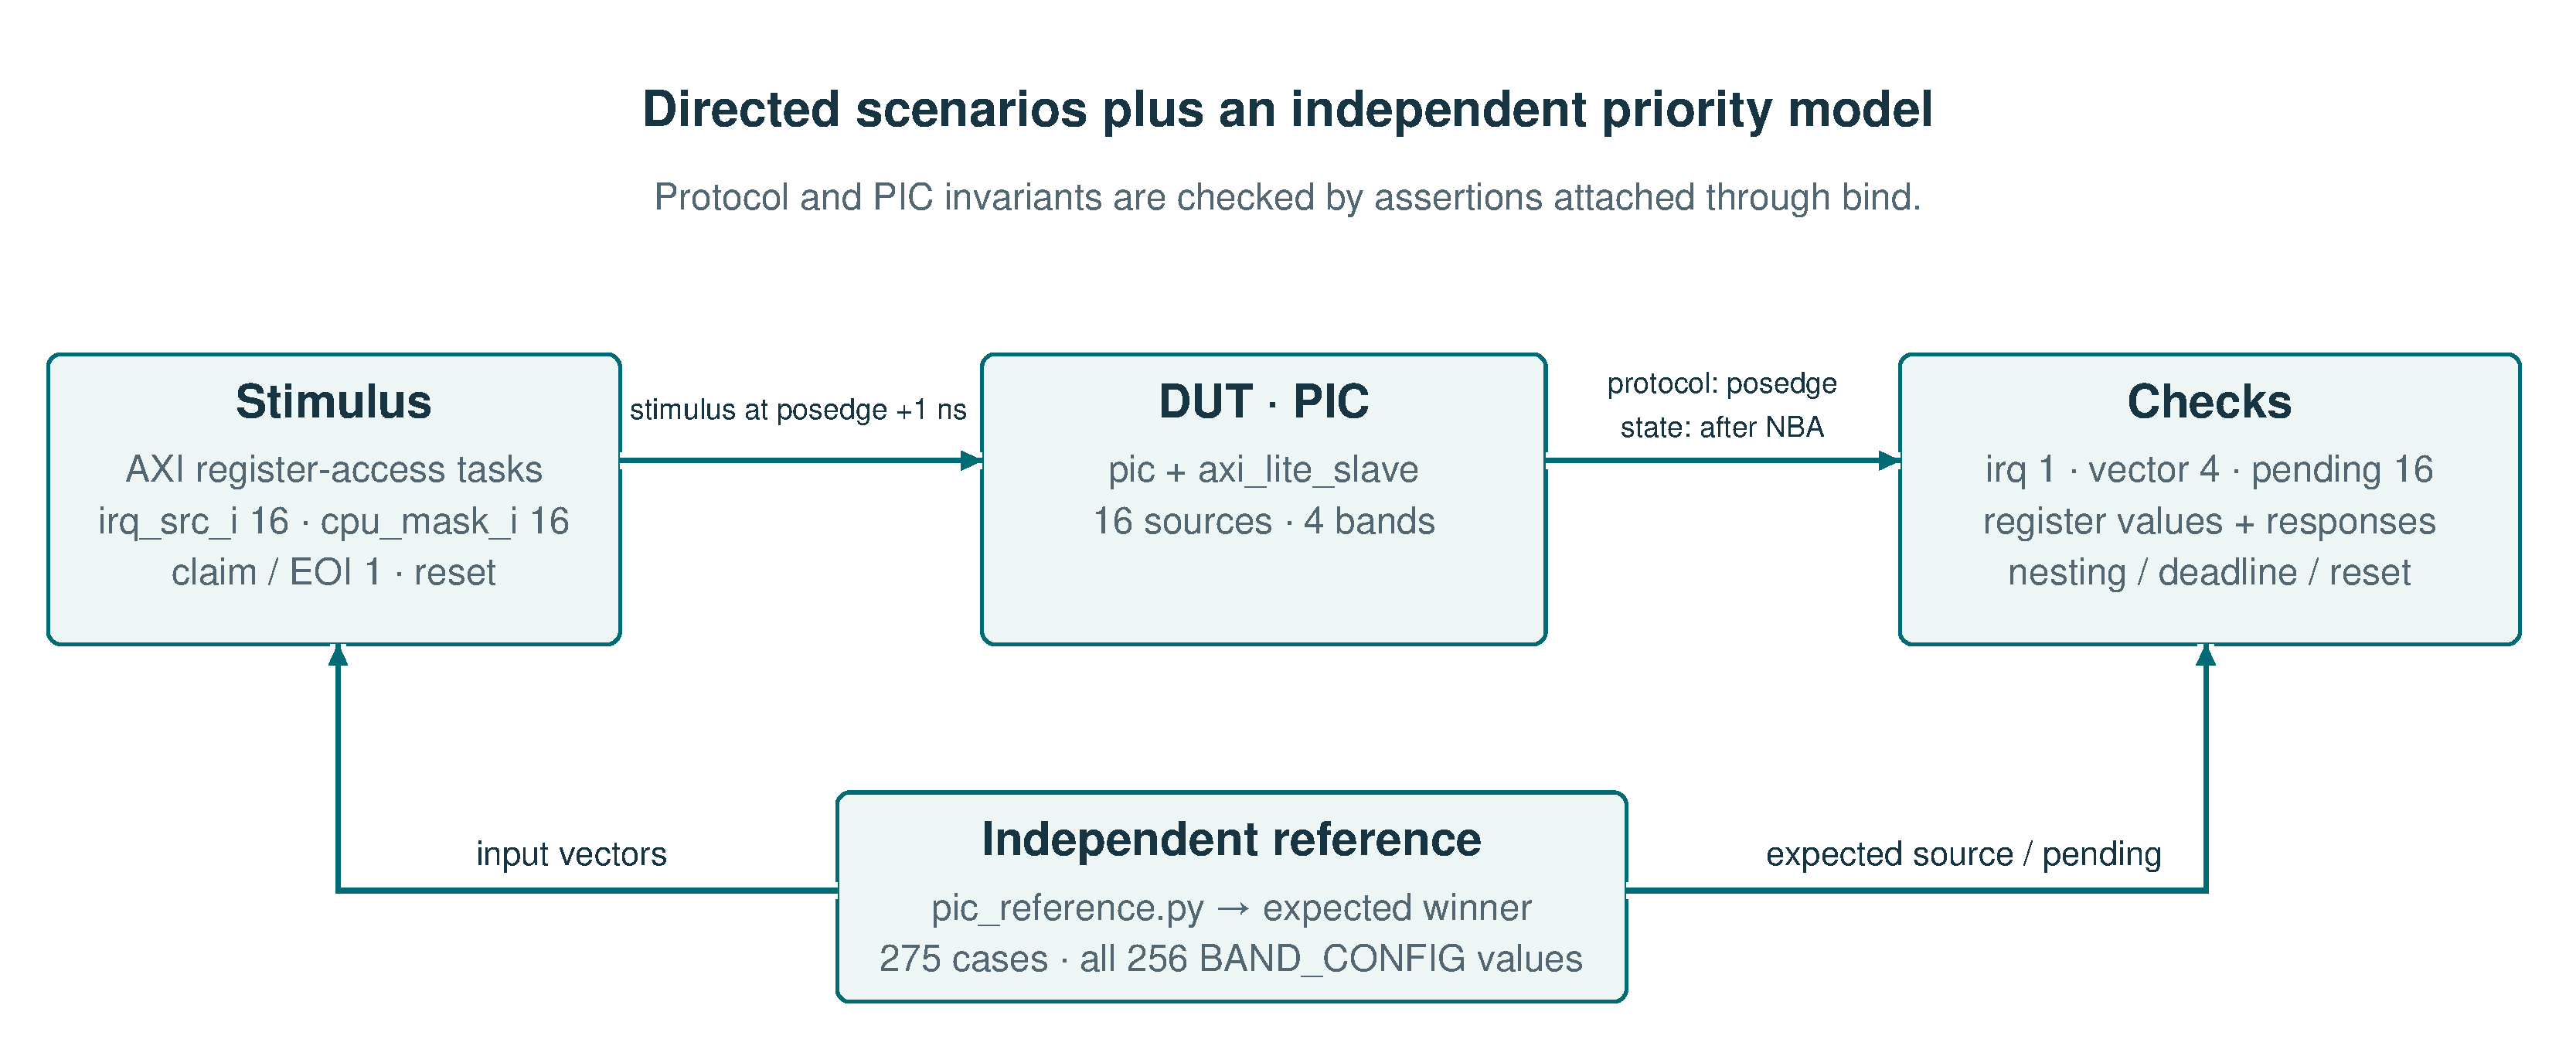
\includegraphics[width=\linewidth,height=105mm,keepaspectratio]{figures/pic_verification.pdf}\caption{Test stimuli, DUT and independent checking paths.}\end{figure}
{\small
\begin{longtable}{@{}L{0.2400\dimexpr\linewidth-12pt\relax}L{0.7600\dimexpr\linewidth-12pt\relax}@{}}
\toprule
\textbf{Component} & \textbf{File / role} \\ \midrule
\endfirsthead
\toprule
\textbf{Component} & \textbf{File / role} \\ \midrule
\endhead
Clock / reset & ck\_rst\_tb.v: shared generator; dedicated reset benches can drive a reset pulse between edges. \\ \addlinespace[3pt]
Bus stimulus & tb\_axil\_master.vh: register-access tasks; CPU programs supply real load/store requests at system level. \\ \addlinespace[3pt]
Memory model & axi\_lite\_mem\_model.v: configurable response delay and repeatable backpressure. \\ \addlinespace[3pt]
Reference & pic\_reference.py: expected priority winner and pending mask. \\ \addlinespace[3pt]
Verdict & tb\_check.vh: explicit mismatch count, completion and fatal failure. \\ \addlinespace[3pt]
Protocol & axi\_lite\_monitor.v for ModelSim; axi\_lite\_sva.sv under Verilator. \\*
\bottomrule\end{longtable}}

\needspace{7\baselineskip}
\subsection{Control and drivers}
\noindent Stimulus is driven one nanosecond after the sampling edge, so that a test never races the design it is checking. The table gives the timing rule for each driven event and the reason for it; the waveform shows the reset case, the one event placed off the clock grid.\par\medskip
{\small
\begin{longtable}{@{}L{0.2400\dimexpr\linewidth-24pt\relax}L{0.4200\dimexpr\linewidth-24pt\relax}L{0.3400\dimexpr\linewidth-24pt\relax}@{}}
\toprule
\textbf{Signal / event} & \textbf{Timing rule} & \textbf{Reason} \\ \midrule
\endfirsthead
\toprule
\textbf{Signal / event} & \textbf{Timing rule} & \textbf{Reason} \\ \midrule
\endhead
clk & 10 ns period in these traces; rising edges are 5, 15, 25… ns. & Defines the handshake observation points. \\ \addlinespace[3pt]
Shared bus / claim tasks & Drive 1 ns after posedge, in a separate statement. Hold until the sampling edge. & Avoid blocking-assignment races with DUT active/NBA evaluation. \\ \addlinespace[3pt]
Handshake observation & Sample VALID \&\& READY at posedge before changing stimulus. & Records the transfer that the DUT accepted. \\ \addlinespace[3pt]
Reset assertion & Dedicated reset tests assert at posedge +2 ns, check at +3 ns. & The check occurs before either the next falling or rising edge. \\ \addlinespace[3pt]
Reset release & Explicit nanosecond delays, off the clock grid; shared generator releases at 123 ns. & Exercises asynchronous stimulus without a coincident clock event. \\*
\bottomrule\end{longtable}}

\noindent The controller starts with active nested service and enabled sources. Reset clears both depth and INT\_ENABLE between clock edges; the test checks the state one nanosecond after assertion.\par
\begin{figure}[H]\centering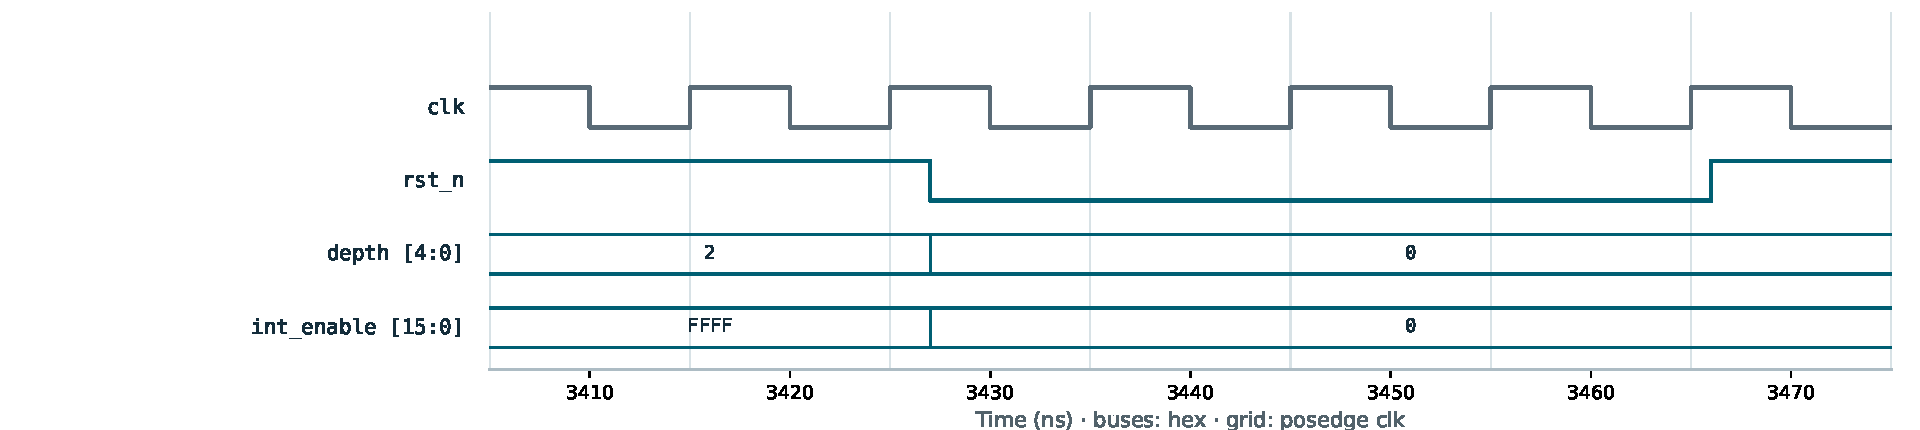
\includegraphics[width=\linewidth]{waves/pic_reset.pdf}\caption{Reset from active state at posedge +2 ns; cleared state is checked at +3 ns.}\end{figure}
\subsubsection{Clock and reset generator}
\noindent ck\_rst\_tb.v generates a 10 ns clock and holds reset from time 0 to 123 ns, off the clock edge. pic\_tb\_reset drives its own reset pulses between edges.\par\medskip
\subsubsection{AXI4-Lite master tasks}
\noindent tb\_axil\_master.vh provides register read and write tasks that check the response code. AW and W are issued together and may complete in either order.\par\medskip
\subsubsection{Source and CPU-side drivers}
\noindent The block benches drive irq\_src\_i, cpu\_mask\_i and the claim/EOI pair directly, in place of the CPU.\par\medskip
\subsubsection{Random traffic}
\noindent pic\_tb\_random draws register writes, sources, masks, claims and EOIs from a seed (+seed, +cycles) and writes every cycle to pic\_random.trace.\par\medskip

\needspace{7\baselineskip}
\subsection{Monitors and checkers}
\noindent Checking is split between bus protocol and functional result, so that a failure points at one of the two.\par\medskip
\subsubsection{AXI protocol monitor}
\noindent axi\_lite\_monitor.v checks every transfer on the monitored ports in ModelSim and counts transactions; a run without traffic fails.\par\medskip
\subsubsection{Assertions}
\noindent axi\_lite\_sva.sv checks the register port; pic\_sva.sv checks offer eligibility, the CPU mask, the priority threshold, depth transitions, claim/EOI exclusion and the empty EOI. rv32i\_bind\_core\_sva.sv attaches the checkers to the RTL module types with bind; they only read DUT signals. Verilator runs them with --assert; ModelSim ASE runs the procedural monitors.\par\medskip
\subsubsection{Result checkers}
\noindent tb\_check.vh counts mismatches and ends each run with an explicit verdict. pic\_tb\_reference compares winner and pending mask with pic\_reference.py; pic\_model.py replays each random trace and compares every cycle.\par\medskip
\subsubsection{Formal harness}
\noindent pic\_formal.sv states the PIC invariants for SymbiYosys. run\_formal.sh runs the proofs, then repeats them with five injected defects, each of which must fail.\par\medskip
\subsubsection{Non-vacuous checks}
{\small
\begin{longtable}{@{}L{0.3200\dimexpr\linewidth-12pt\relax}L{0.6800\dimexpr\linewidth-12pt\relax}@{}}
\toprule
\textbf{Non-vacuous check} & \textbf{Evidence} \\ \midrule
\endfirsthead
\toprule
\textbf{Non-vacuous check} & \textbf{Evidence} \\ \midrule
\endhead
Valid traffic & Read/write counts and exercised tests prevent a disconnected monitor from being counted as coverage. \\ \addlinespace[3pt]
Preconditions & RO-write test first creates nonzero state; async-reset test first creates pending/nonzero state. \\ \addlinespace[3pt]
Negative scenarios & Watch an interval for forbidden offers/claims; do not infer absence from one sample. \\*
\bottomrule\end{longtable}}

\needspace{7\baselineskip}
\subsection{Simulation environment setup}
\noindent The environment is a fixed folder layout plus a small number of named scripts. The tables give that layout, the exact command for each step in the order it is run, and the tools each step needs.\par\medskip
\needspace{7\baselineskip}\subsubsection{Structure}
{\small
\begin{longtable}{@{}L{0.2200\dimexpr\linewidth-12pt\relax}L{0.7800\dimexpr\linewidth-12pt\relax}@{}}
\toprule
\textbf{Folder} & \textbf{Contents} \\ \midrule
\endfirsthead
\toprule
\textbf{Folder} & \textbf{Contents} \\ \midrule
\endhead
cpu/hdl & Synthesizable RTL: the CPU modules, the PIC, the timer and the AXI4-Lite register front-end. \\ \addlinespace[3pt]
cpu/debug/hdl & Testbenches, bus masters and the configurable memory and responder models. \\ \addlinespace[3pt]
cpu/debug/sva & Assertion modules and the bind files that attach them to RTL module types. \\ \addlinespace[3pt]
cpu/debug/sim & Run scripts, file lists, reference models, generated programs and run logs. \\ \addlinespace[3pt]
soc/hdl & Integration fabric: address decode, arbitration, AXI4-Full to Lite conversion and RAM. \\ \addlinespace[3pt]
soc/debug/hdl, sva, sim & The same split as above, applied to the integrated SoC. \\ \addlinespace[3pt]
cpu/docs & Specification sources, generated figures and the waveform windows. \\*
\bottomrule\end{longtable}}
\needspace{7\baselineskip}\subsubsection{Scripts}
{\small
\begin{longtable}{@{}L{0.0600\dimexpr\linewidth-36pt\relax}L{0.2200\dimexpr\linewidth-36pt\relax}L{0.4300\dimexpr\linewidth-36pt\relax}L{0.2900\dimexpr\linewidth-36pt\relax}@{}}
\toprule
\textbf{Step} & \textbf{Working directory} & \textbf{Command / script} & \textbf{Result} \\ \midrule
\endfirsthead
\toprule
\textbf{Step} & \textbf{Working directory} & \textbf{Command / script} & \textbf{Result} \\ \midrule
\endhead
1 & Repository root & make asm & Regenerate programs and independent reference vectors. \\ \addlinespace[3pt]
2 & cpu/debug/sim & vsim -c -do "do regress.do; quit -f" & Compile and run 39 CPU/PIC runs. \\ \addlinespace[3pt]
3 & cpu/debug/sim (Bash / WSL) & bash run\_verilator.sh & Lint, 17 benches in 53 runs with SVA, coverage and cover gates. \\ \addlinespace[3pt]
4 & soc/debug/sim & vsim -c -do "do regress.do; quit -f" & 34 integration runs. \\ \addlinespace[3pt]
5 & Repository root (Bash / WSL) & bash soc/debug/sim/run\_verilator.sh & SoC lint and 23 assertion-enabled benches in 51 runs. \\ \addlinespace[3pt]
6 & soc/debug/sim (Bash / WSL) & bash run\_pulp\_compare.sh & Pinned external decoder/register comparison. \\ \addlinespace[3pt]
7 & Repository root (Bash / WSL) & bash cpu/debug/formal/run\_formal.sh & PIC proofs, then the injected defects. \\ \addlinespace[3pt]
8 & Repository root & python cpu/debug/sim/mutation\_check.py & 25 injected RTL defects. \\ \addlinespace[3pt]
9 & cpu/debug/sim & vsim -c -do "do waves.do" & Run 8 checked benches and export VCD traces. \\ \addlinespace[3pt]
10 & Repository root & python cpu/docs/tools/waveforms.py & SVG/PDF/PNG figures and source-window manifest. \\*
\bottomrule\end{longtable}}
\needspace{7\baselineskip}\subsubsection{Setup and configuration}
{\small
\begin{longtable}{@{}L{0.2600\dimexpr\linewidth-12pt\relax}L{0.7400\dimexpr\linewidth-12pt\relax}@{}}
\toprule
\textbf{Tool / setup} & \textbf{Requirement} \\ \midrule
\endfirsthead
\toprule
\textbf{Tool / setup} & \textbf{Requirement} \\ \midrule
\endhead
ModelSim & vsim/vlog on PATH; run from the named simulation directory so file lists resolve. \\ \addlinespace[3pt]
Verilator & Verilator 5.050 used for the recorded run; C++ build tools, Bash and Python 3 are required. \\ \addlinespace[3pt]
PULP & Git and network only for the initial checkout; explicit revision pins recorded in the runner. \\ \addlinespace[3pt]
SymbiYosys & yosys, sby, yosys-abc and z3 on PATH. \\ \addlinespace[3pt]
Wave rendering & Python with matplotlib; raw VCD files produced by waves.do. \\ \addlinespace[3pt]
Configuration & Latency/stall overrides are read back after elaboration; seeds are fixed for repeatability. \\*
\bottomrule\end{longtable}}

\clearpage
\section{Annex}
\subsection{Verification plan}
\noindent PASS indicates the recorded regression completed with its expected results and zero checker errors. Each row identifies the test that exercises the listed behavior.\par\medskip
{\small
\begin{longtable}{@{}L{0.0800\dimexpr\linewidth-48pt\relax}L{0.1600\dimexpr\linewidth-48pt\relax}L{0.3700\dimexpr\linewidth-48pt\relax}L{0.1000\dimexpr\linewidth-48pt\relax}L{0.2900\dimexpr\linewidth-48pt\relax}@{}}
\toprule
\textbf{ID} & \textbf{Title} & \textbf{Description} & \textbf{Status} & \textbf{Test / checker} \\ \midrule
\endfirsthead
\toprule
\textbf{ID} & \textbf{Title} & \textbf{Description} & \textbf{Status} & \textbf{Test / checker} \\ \midrule
\endhead
PIC-01 & Feature sequences & Level/edge sources, priority bands/intra-band/ties, nesting, limit, spurious, escalation, SW trigger and access response codes. & PASS & pic\_tb\_feature \\ \addlinespace[3pt]
PIC-02 & Priority reference & Independent priority model: 275 cases covering all 256 BAND\_CONFIG encodings, request/enable/CPU masks and ties. & PASS & pic\_tb\_reference \\ \addlinespace[3pt]
PIC-03 & Simultaneous events & Masked source cannot starve another; fresh edge coincident with claim; reordered-band escalation; trigger-key strobes. & PASS & pic\_tb\_sched \\ \addlinespace[3pt]
PIC-04 & Asynchronous reset & All per-source/global defaults, loaded-state reset before next clock edge, reset with AW-only/W-only/B-held/R-held, recovery. & PASS & pic\_tb\_reset \\ \addlinespace[3pt]
PIC-05 & Read-only registers & Write every RO register from a nonzero hardware state; expect SLVERR and unchanged value. & PASS & pic\_tb\_ro \\ \addlinespace[3pt]
PIC-06 & Status transitions & PEND, ACTIVE, ESC, SPUR, EFF\_BAND and timer fields; exact escalation transitions and complete source life cycle. & PASS & pic\_tb\_status \\ \addlinespace[3pt]
PIC-07 & CPU integration & CPU programs the real PIC; claim/EOI order, masks, pending and interrupt handling across LSU stalls. & PASS & rv32i\_tb\_cpu\_axi \\ \addlinespace[3pt]
PIC-08 & SoC integration & Interrupt source routing, nesting to sixteen levels, escalation and a spurious claim with the real CPU in the integrated SoC. & PASS & soc\_tb\_pic\_sources / nest / escalate / spurious / deep\_nest \\ \addlinespace[3pt]
PIC-09 & Random traffic & Random register writes, sources, masks, claims and EOIs, reconfiguration while nested included; every cycle equal to the cycle model pic\_model.py. & PASS & pic\_tb\_random \\ \addlinespace[3pt]
PIC-10 & Formal proofs & Proven for every input: stack depth at most 16, NEST\_MAX in 1..16, a claim at the limit and an EOI on an empty stack change nothing, software requests only through a keyed write, only eligible sources offered; five injected defects each fail the proof. & PASS & pic\_formal.sv (SymbiYosys) \\*
\bottomrule\end{longtable}}

\needspace{7\baselineskip}
\subsection{Critical sequences}

\noindent A second source edge is sampled with the claim of the first event. The edge latch remains set, and the source is offered again after EOI.\par
\begin{figure}[H]\centering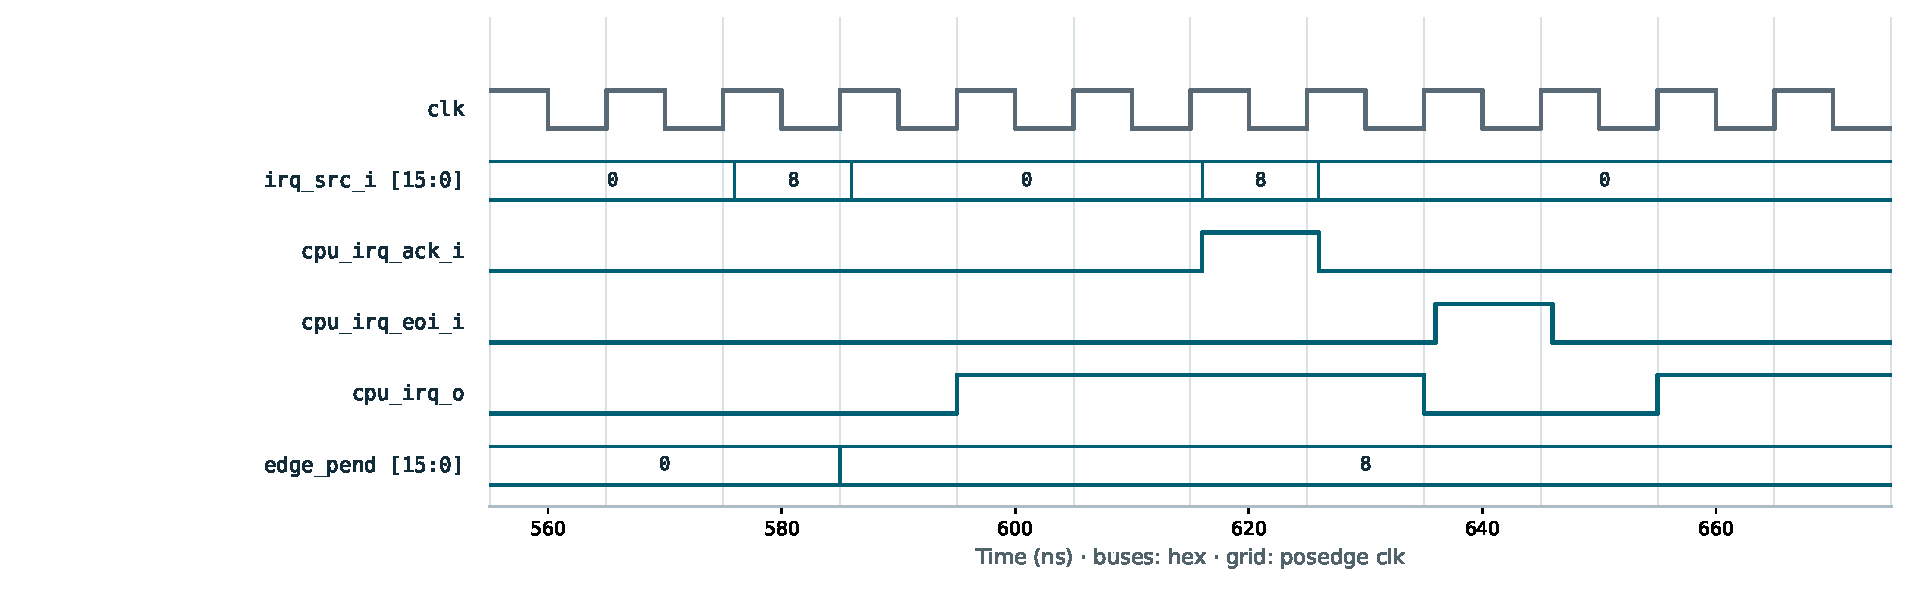
\includegraphics[width=\linewidth]{waves/pic_edge_claim.pdf}\caption{New edge coincident with claim: the edge latch remains set.}\end{figure}

\noindent Source 1 initially wins the tie. Source 2 reaches its ten-cycle deadline; the escalation event changes its effective priority, and the registered offer changes to source 2 on the following edge.\par
\begin{figure}[H]\centering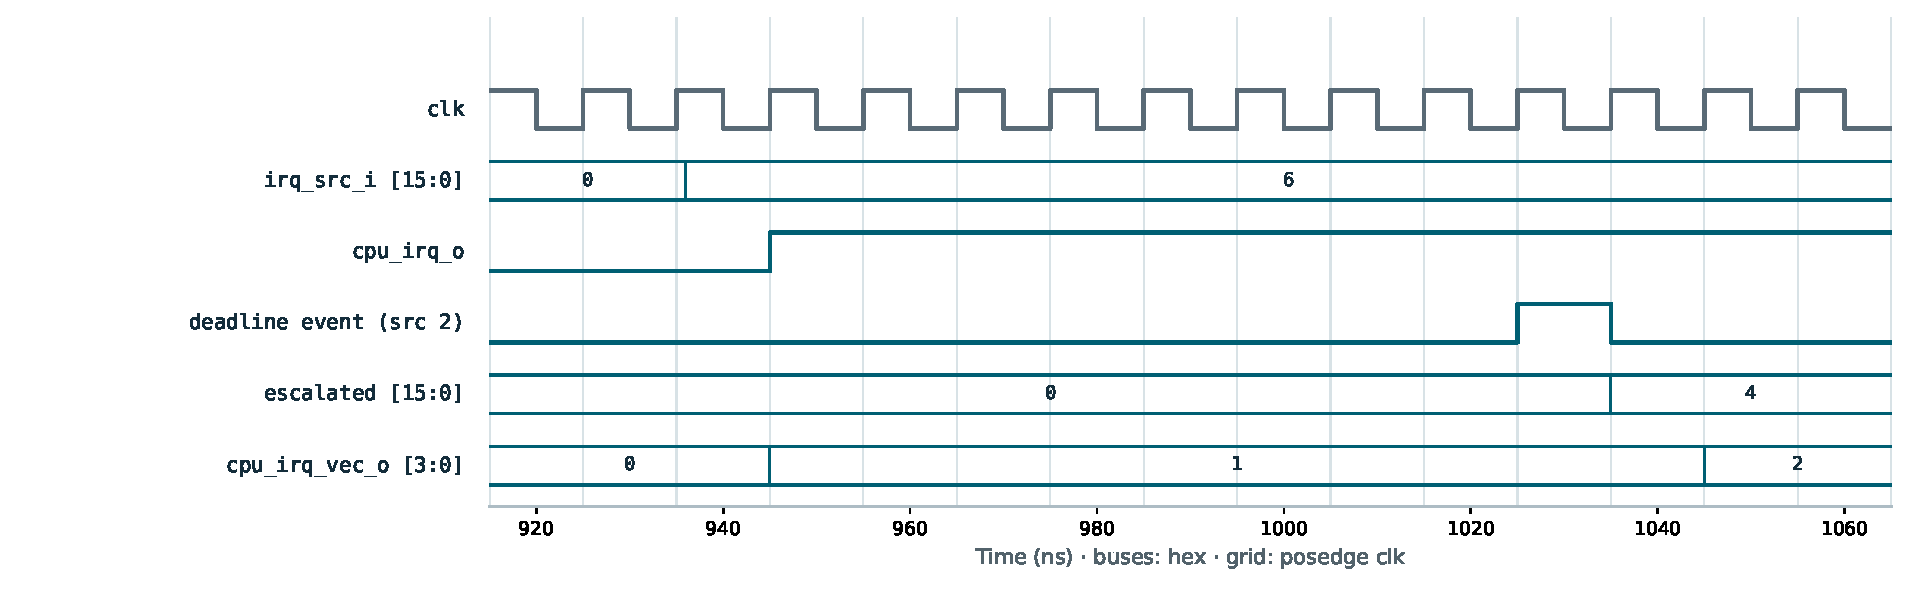
\includegraphics[width=\linewidth]{waves/pic_escalation.pdf}\caption{Ten-cycle deadline: escalation event, then registered source 2 offer under reordered band urgency.}\end{figure}
{\small
\begin{longtable}{@{}L{0.3000\dimexpr\linewidth-12pt\relax}L{0.7000\dimexpr\linewidth-12pt\relax}@{}}
\toprule
\textbf{Scenario} & \textbf{Check} \\ \midrule
\endfirsthead
\toprule
\textbf{Scenario} & \textbf{Check} \\ \midrule
\endhead
New edge + claim & Old event is consumed, new event is retained. \\ \addlinespace[3pt]
Band reordering & Escalation follows programmed urgency, not numeric band order. \\ \addlinespace[3pt]
Nest limit + eligible source & Offer suppressed and overflow logged; existing stack is preserved. \\*
\bottomrule\end{longtable}}

\needspace{7\baselineskip}
\subsection{External AXI reference}
\noindent The AXI4-Lite front-end is compared against a published implementation to check the interpretation of the protocol. The first table states what was compared and on what evidence; the second names every difference found and what it means.\par\medskip
{\small
\begin{longtable}{@{}L{0.3200\dimexpr\linewidth-24pt\relax}L{0.3500\dimexpr\linewidth-24pt\relax}L{0.3300\dimexpr\linewidth-24pt\relax}@{}}
\toprule
\textbf{Compared block} & \textbf{Shared contract} & \textbf{Evidence} \\ \midrule
\endfirsthead
\toprule
\textbf{Compared block} & \textbf{Shared contract} & \textbf{Evidence} \\ \midrule
\endhead
soc\_axi\_lite\_dec vs axi\_lite\_demux & Two mapped targets, MaxTrans=1; independent progress and response timing. & Compare ordered data/response records and per-target address counts. \\ \addlinespace[3pt]
axi\_lite\_slave vs axi\_lite\_regs & 32-bit words; four RW words and one RO word; same byte strobes. & 96 cases = 16 WSTRB masks × 3 AW/W orders × 2 response-stall settings. \\ \addlinespace[3pt]
Additional register cases & RO write, unmapped access, reset and post-reset access. & Same access-class response and no forbidden state update; each side checked against expected data. \\*
\bottomrule\end{longtable}}
{\small
\begin{longtable}{@{}L{0.2500\dimexpr\linewidth-12pt\relax}L{0.7500\dimexpr\linewidth-12pt\relax}@{}}
\toprule
\textbf{Difference / boundary} & \textbf{Interpretation} \\ \midrule
\endfirsthead
\toprule
\textbf{Difference / boundary} & \textbf{Interpretation} \\ \midrule
\endhead
Latency & Not cycle-identical; compare completed transactions and protocol compliance. \\ \addlinespace[3pt]
Unmapped read data & Our front-end returns zero; pinned PULP axi\_lite\_regs returns 0xBA5E1E55. Both return SLVERR; error-data policy is documented separately. \\ \addlinespace[3pt]
Address aliases & Different register-bank sizing; equality claimed only for the explicit compared address profile. \\ \addlinespace[3pt]
AXI4-Full & The PULP run does not establish equivalence of the DMA or soc\_axi\_full2lite to every upstream AXI4 module. \\ \addlinespace[3pt]
Converter & Local soc\_tb\_full2lite and soc\_tb\_full2lite\_err check supported burst handling and errors. Local write error aggregation preserves DECERR over SLVERR; PULP is not a cycle-exact reference for that policy. \\ \addlinespace[3pt]
Versions & axi: 70b8e54fd460e3308e58be596ceb3566a6e3576e; common\_cells: 03d98106aa19952a10360d2230def85144a0008b. \\*
\bottomrule\end{longtable}}
\noindent Reference: \url{https://github.com/pulp-platform/axi}.

\end{document}
